\documentclass[11pt]{article}

\usepackage[margin=1in]{geometry}
\usepackage{amsmath,amssymb}
\usepackage{booktabs}
\usepackage{graphicx}
\usepackage{subcaption}
\usepackage{hyperref}

\graphicspath{{images/}}
\hypersetup{
  colorlinks=true,
  linkcolor=blue,
  urlcolor=blue,
  citecolor=blue
}

\title{CS728 Programming Assignment 2}
% \author{Kshitij Vaidya}

\begin{document}
\maketitle

% \section{Setup}
% This report follows the required regimes in \texttt{CS728\_2026\_Programming\_Assignment\_2.pdf}:
% \begin{itemize}
%   \item Task 1 (A1--A5): Memorization (\texttt{mem}), sequence-level classification at every time step (\texttt{classifType=softmax}).
%   \item Task 2 (B1--B2): Multiplication (\texttt{mul}), regression from the final hidden state (\texttt{classifType=lastLinear}).
%   \item All runs use the common flags from the PDF (hidden size 50, length 50--200, SGD updates up to 50k, diagnostics enabled).
% \end{itemize}

% \section{Diagnostics and Interpretation}
% The report answers Q1--Q5 using the following logged diagnostics at the final checkpoint:
% \begin{itemize}
%   \item \textbf{Gradient-through-time signal:} $g_t = \mathbb{E}_\text{batch}\|\partial L/\partial h_t\|_2$, plotted as a histogram of $\log_{10}(g_t+\varepsilon)$ across time steps.
%   Very negative values (e.g.\ $-8$ to $-12$) indicate vanishing gradients across time.
%   \item \textbf{Hidden saturation distance:} for tanh states $h_t\in[-1,1]$, $d(h)=1-|h|$ and the plotted histogram is over time steps of $\mathbb{E}[d(h_t)]$.
%   Small values (near $0$) indicate saturation near $\pm 1$; large values indicate activations closer to $0$ (unsaturated).
%   \item \textbf{GRU gate saturation distance:} for gates $v\in[0,1]$, $d(v)=\min(v,1-v)$.
%   Here $d\approx 0$ means the gate is saturated near $0$ or $1$, while $d\approx 0.5$ indicates an unsaturated gate near $0.5$.
%   \item \textbf{Global gradient norm:} $\|\nabla_\theta L\|_2$ over training. For clipped runs (rescale clipping), the post-clip norm is reconstructed as $\min(\|\nabla_\theta L\|_2,\texttt{cutoff})$.
%   \item \textbf{Spectral radius proxy:} $\rho(W_{hh})$ over training, computed from the recurrent matrix exposed by the model.
% \end{itemize}

\section{Summary Table}


\begin{table}[h]
  \centering
  \begin{tabular}{lllcccccc}
\toprule
Run & Task & Model & Clip & $\log_{10}\|dL/dh_t\|$ & $\mu_{sat}$ & $sat<0.05$(\%) & $\rho(W_{hh})$ (last) & bestValidErr(\%) \\
\midrule
A1 & mem & RNN & none & -4.22 & 0.017 & 99.5 & 14.20 & 100.00 \\
A2 & mem & RNN & 0.05 & -4.58 & 0.628 & 0.0 & 1.14 & 100.00 \\
A3 & mem & RNN & 0.01 & -4.60 & 0.611 & 0.0 & 1.12 & 100.00 \\
A4 & mem & GRU & none & -6.07 & 0.538 & 0.0 & 2.01 & 100.00 \\
A5 & mem & GRU & 0.05 & -4.18 & 0.850 & 0.0 & 1.29 & 100.00 \\
B1 & mul & RNN & none & -12.00 & 0.939 & 0.0 & 0.71 & 25.90 \\
B2 & mul & GRU & none & -12.00 & 0.995 & 0.0 & 0.08 & 24.25 \\
\bottomrule
\end{tabular}

  \caption{Per Run Summary}
\end{table}

\section{Results: Memorization (A1--A5)}

\subsection{A1: RNN (tanh), no clipping}
\begin{figure}[h]
  \centering
  \begin{subfigure}{0.32\textwidth}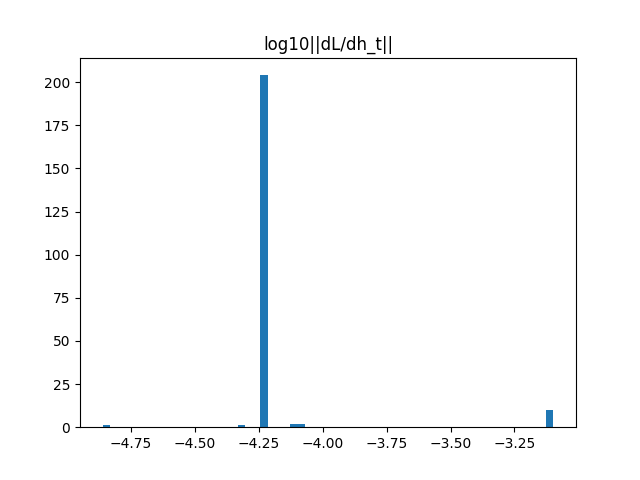
\includegraphics[width=\linewidth]{A1_mem_rnn_tanh_noclip_hist.png}\caption{$\log_{10}\|dL/dh_t\|$}\end{subfigure}
  \begin{subfigure}{0.32\textwidth}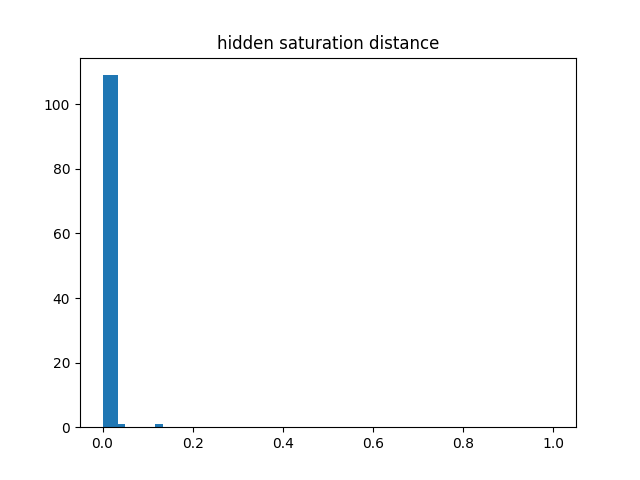
\includegraphics[width=\linewidth]{A1_mem_rnn_tanh_noclip_hidden_sat_dist.png}\caption{hidden sat distance}\end{subfigure}
  \begin{subfigure}{0.32\textwidth}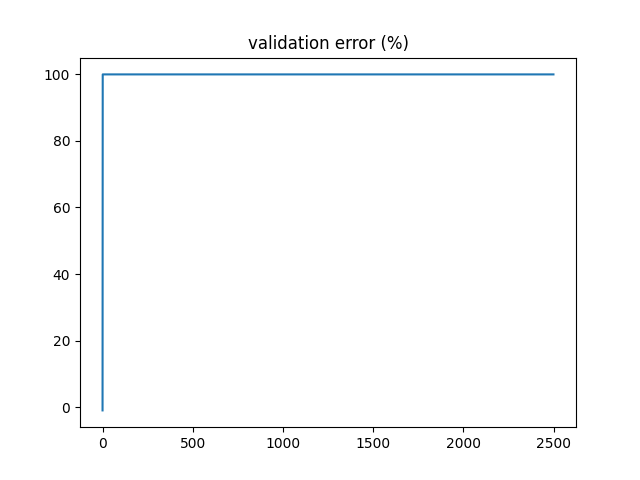
\includegraphics[width=\linewidth]{A1_mem_rnn_tanh_noclip_val_err.png}\caption{valid error}\end{subfigure}
  \caption{A1 diagnostics.}
  \label{fig:a1}
\end{figure}
\noindent\textbf{Q1 (vanish/explode?):} $\log_{10}\|dL/dh_t\|$ is concentrated around $\approx -4.2$, so the gradient-through-time signal is not extremely vanishing (not near $-8$ to $-12$) and not exploding.\\
\textbf{Q2 (saturation?):} hidden saturation distance mass is extremely close to $0$ (Table~\ref{tab:summary}: $99.5\%$ of time steps have sat-distance $<0.05$), indicating strong tanh saturation. This saturation co-occurs with a very large $\rho(W_{hh})$ (final $\approx 14.2$), suggesting unstable recurrent dynamics where saturation can suppress useful learning signals even if $g_t$ is not numerically tiny.\\
\textbf{Validation:} validation error remains at $100\%$ throughout, so the model does not learn the memorization task in this regime.

\subsection{A2: RNN (tanh), clipping cutoff 0.05}
\begin{figure}[h]
  \centering
  \begin{subfigure}{0.32\textwidth}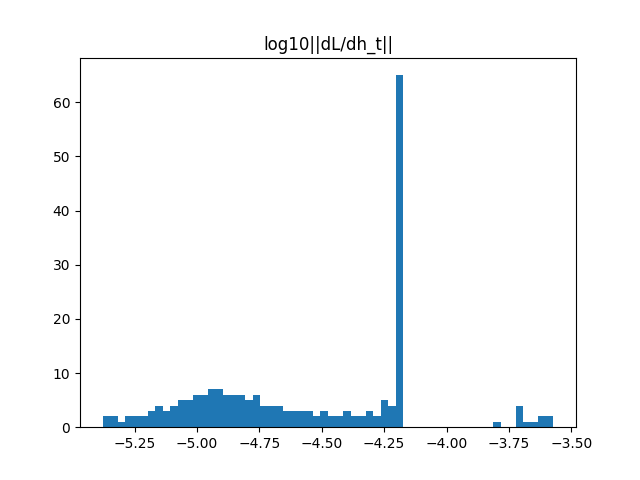
\includegraphics[width=\linewidth]{A2_mem_rnn_tanh_clip005_hist.png}\caption{$\log_{10}\|dL/dh_t\|$}\end{subfigure}
  \begin{subfigure}{0.32\textwidth}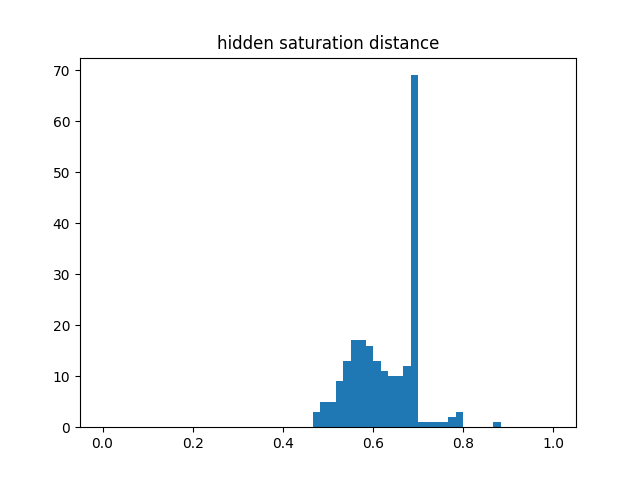
\includegraphics[width=\linewidth]{A2_mem_rnn_tanh_clip005_hidden_sat_dist.png}\caption{hidden sat distance}\end{subfigure}
  \begin{subfigure}{0.32\textwidth}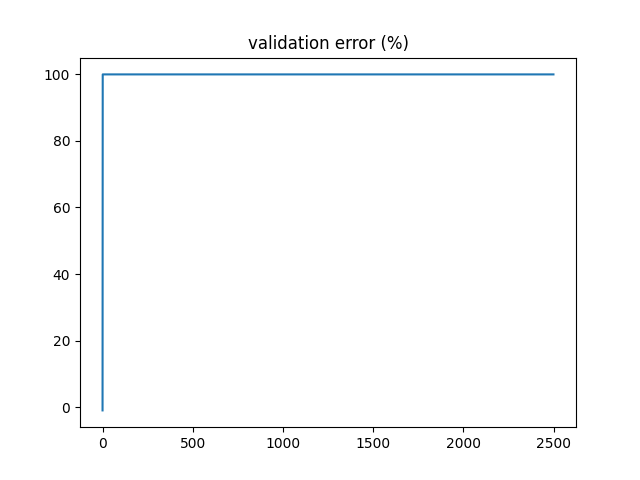
\includegraphics[width=\linewidth]{A2_mem_rnn_tanh_clip005_val_err.png}\caption{valid error}\end{subfigure}
  \caption{A2 diagnostics.}
  \label{fig:a2}
\end{figure}
\noindent\textbf{Q1:} the histogram shifts slightly more negative than A1 (median $\approx -4.6$), but it is still far from the extreme vanishing regime.\\
\textbf{Q2:} saturation largely disappears (mean sat-distance $\approx 0.63$; sat$<0.05\%=0$), indicating hidden states mostly remain in the linear region of tanh.
This shows that strong saturation is \emph{not} necessary for failure on this task.\\
\textbf{Validation:} validation error stays at $100\%$.

\subsection{A3: RNN (tanh), clipping cutoff 0.01}
\begin{figure}[h]
  \centering
  \begin{subfigure}{0.32\textwidth}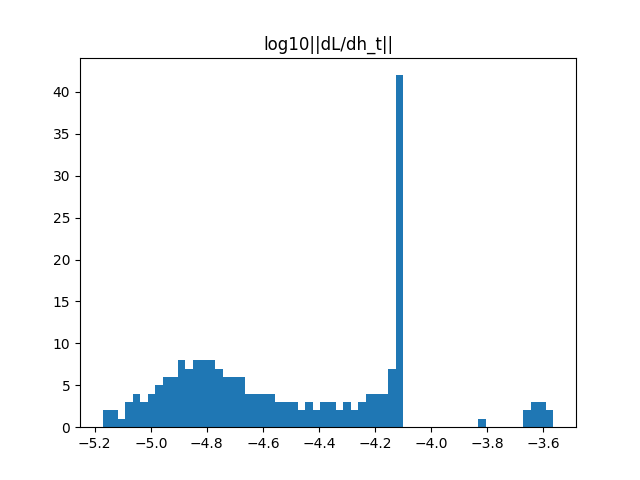
\includegraphics[width=\linewidth]{A3_mem_rnn_tanh_clip001_hist.png}\caption{$\log_{10}\|dL/dh_t\|$}\end{subfigure}
  \begin{subfigure}{0.32\textwidth}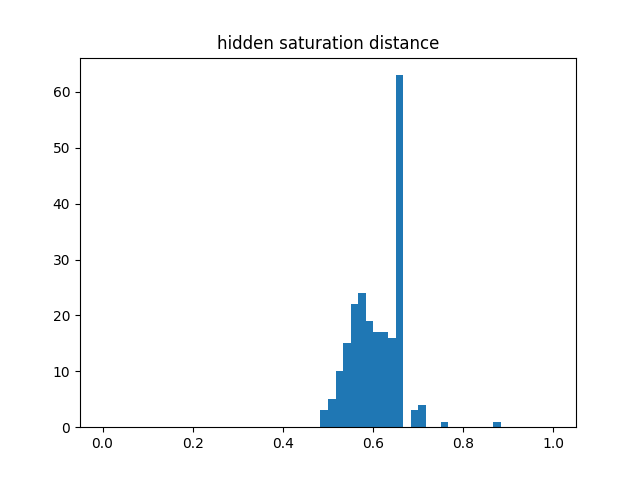
\includegraphics[width=\linewidth]{A3_mem_rnn_tanh_clip001_hidden_sat_dist.png}\caption{hidden sat distance}\end{subfigure}
  \begin{subfigure}{0.32\textwidth}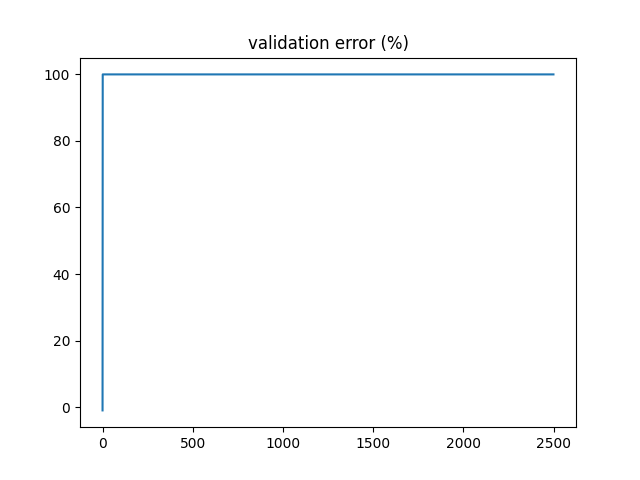
\includegraphics[width=\linewidth]{A3_mem_rnn_tanh_clip001_val_err.png}\caption{valid error}\end{subfigure}
  \caption{A3 diagnostics.}
  \label{fig:a3}
\end{figure}
\noindent\textbf{Q1:} similar to A2 (median $\approx -4.6$), indicating neither extreme vanishing nor explosion in the $g_t$ histogram.\\
\textbf{Q2:} similar non-saturated hidden behavior to A2 (mean sat-distance $\approx 0.61$).\\
\textbf{Validation:} validation error stays at $100\%$.

\subsection{A4: GRU, no clipping (gate diagnostics)}
\begin{figure}[h]
  \centering
  \begin{subfigure}{0.32\textwidth}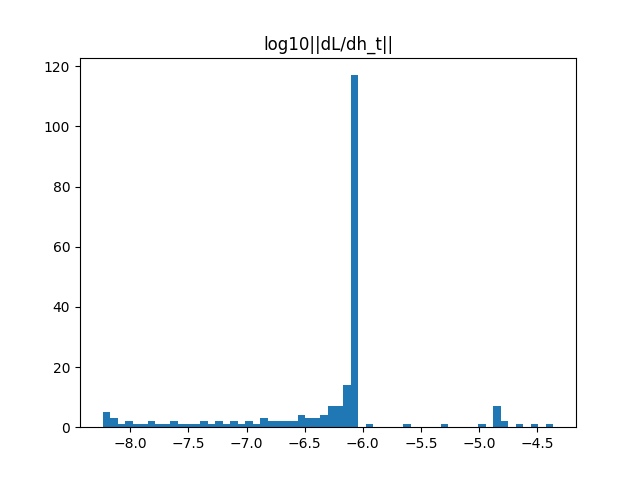
\includegraphics[width=\linewidth]{A4_mem_gru_noclip_hist.png}\caption{$\log_{10}\|dL/dh_t\|$}\end{subfigure}
  \begin{subfigure}{0.32\textwidth}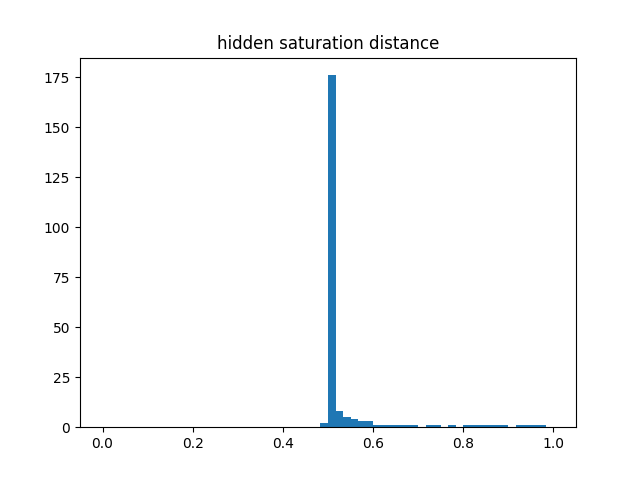
\includegraphics[width=\linewidth]{A4_mem_gru_noclip_hidden_sat_dist.png}\caption{hidden sat distance}\end{subfigure}
  \begin{subfigure}{0.32\textwidth}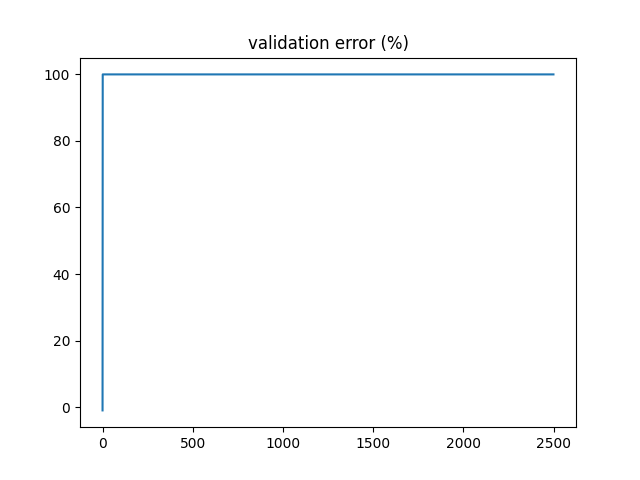
\includegraphics[width=\linewidth]{A4_mem_gru_noclip_val_err.png}\caption{valid error}\end{subfigure}
  \caption{A4 diagnostics.}
  \label{fig:a4}
\end{figure}
\noindent\textbf{Q1:} compared to the RNN runs, the GRU shows substantially more negative values (median $\approx -6.1$ with a tail to $\approx -8$), indicating stronger gradient vanishing across time.\\
\textbf{Q2:} hidden saturation distance is centered around $\approx 0.54$ (not saturated).
Therefore, vanishing gradients can occur even when tanh units are not close to $\pm 1$.\\
\textbf{Q4 (gate saturation):} Figure~\ref{fig:a4gates} shows gate saturation distances.
The update gate has mean $d(z_t)\approx 0.182$ (closer to saturation than $0.5$), while the reset gate is largely unsaturated with mean $d(r_t)\approx 0.456$ (near $0.5$).
This suggests the GRU is often operating with a somewhat saturated update gate, but this alone does not prevent gradient vanishing in this regime.\\
\textbf{Validation:} validation error stays at $100\%$.

\begin{figure}[h]
  \centering
  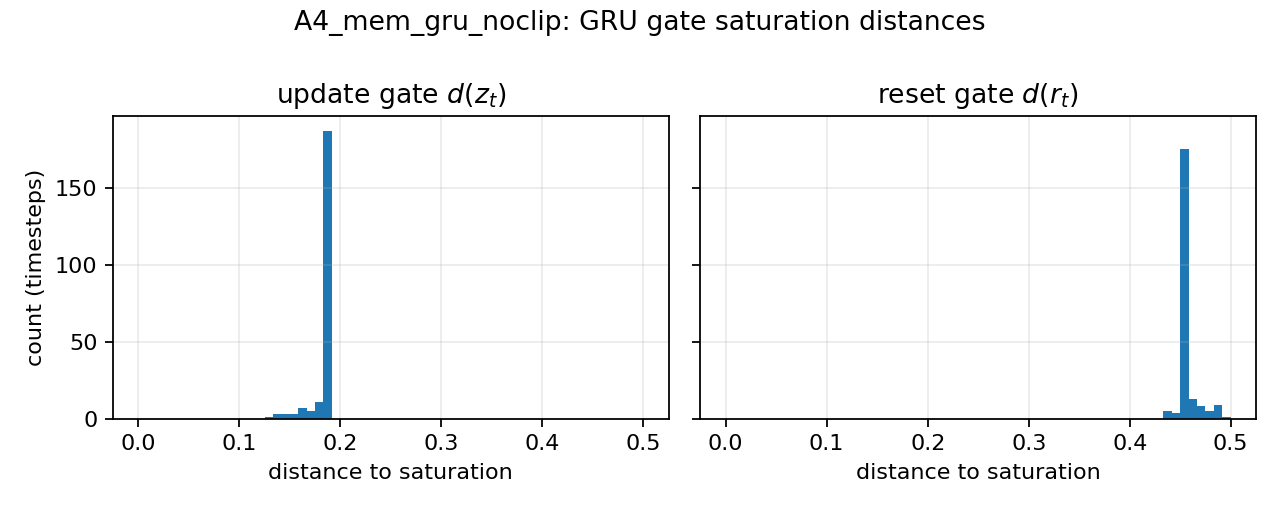
\includegraphics[width=0.85\textwidth]{A4_mem_gru_noclip_gate_sat_hist.png}
  \caption{A4 GRU gate saturation-distance histograms.}
  \label{fig:a4gates}
\end{figure}

\subsection{A5: GRU, clipping cutoff 0.05 (gate diagnostics)}
\begin{figure}[h]
  \centering
  \begin{subfigure}{0.32\textwidth}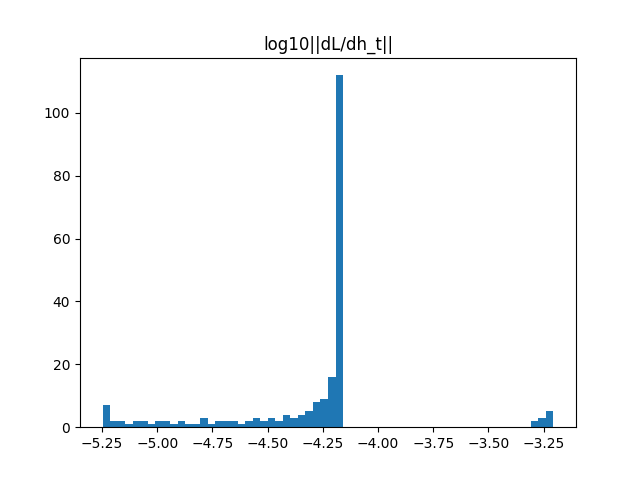
\includegraphics[width=\linewidth]{A5_mem_gru_clip005_hist.png}\caption{$\log_{10}\|dL/dh_t\|$}\end{subfigure}
  \begin{subfigure}{0.32\textwidth}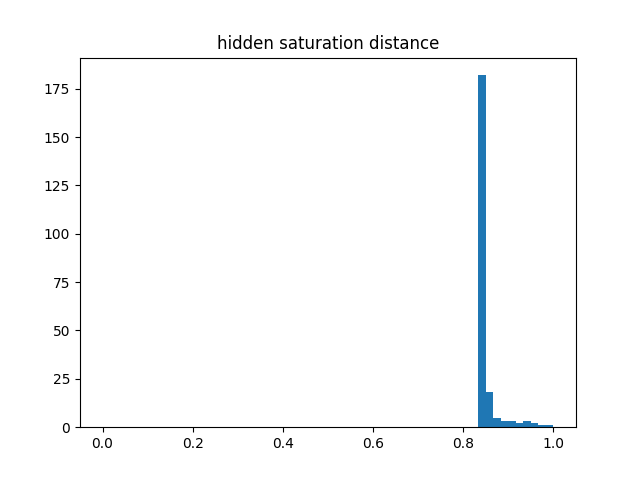
\includegraphics[width=\linewidth]{A5_mem_gru_clip005_hidden_sat_dist.png}\caption{hidden sat distance}\end{subfigure}
  \begin{subfigure}{0.32\textwidth}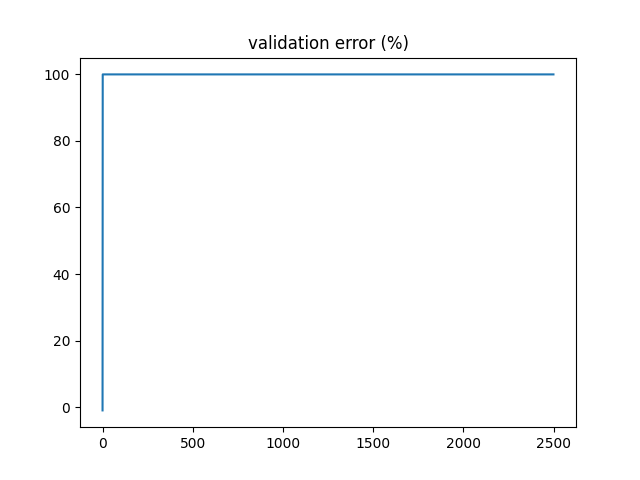
\includegraphics[width=\linewidth]{A5_mem_gru_clip005_val_err.png}\caption{valid error}\end{subfigure}
  \caption{A5 diagnostics.}
  \label{fig:a5}
\end{figure}
\noindent\textbf{Q1:} clipping shifts the GRU $g_t$ histogram towards larger values (median $\approx -4.2$), i.e.\ much less vanishing than A4.\\
\textbf{Q2:} hidden saturation distance moves close to $1$ (mean $\approx 0.85$), indicating hidden states are very close to $0$ (strongly unsaturated).\\
\textbf{Q4 (gate saturation):} Figure~\ref{fig:a5gates} shows that the update gate becomes even more saturated (mean $d(z_t)\approx 0.125$), while the reset gate remains mostly unsaturated (mean $d(r_t)\approx 0.492$).\\
\textbf{Validation:} validation error stays at $100\%$ despite improved gradient-through-time diagnostics.

\begin{figure}[h]
  \centering
  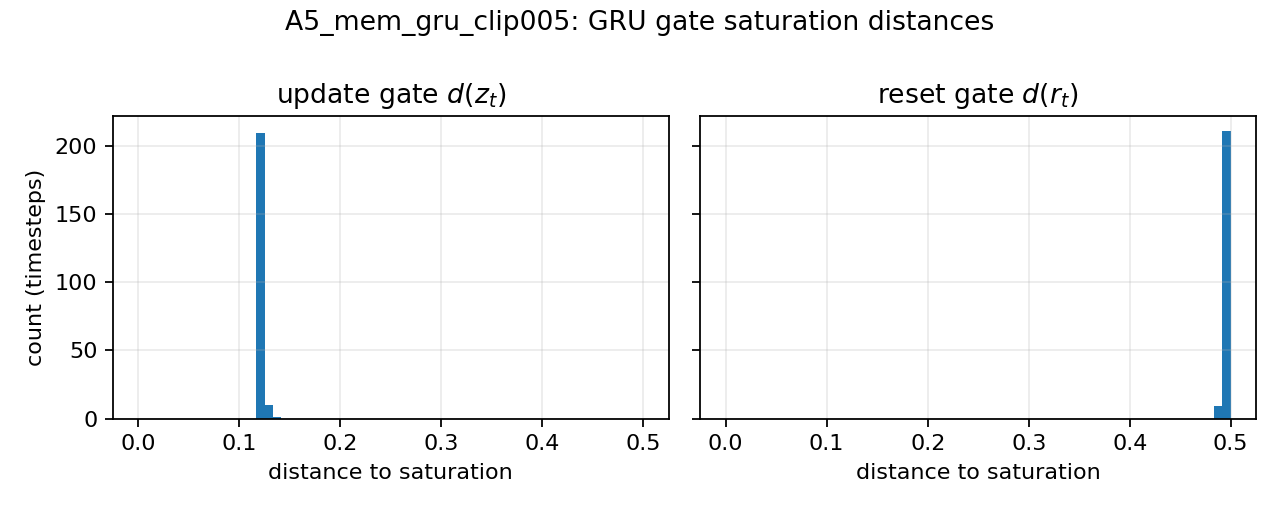
\includegraphics[width=0.85\textwidth]{A5_mem_gru_clip005_gate_sat_hist.png}
  \caption{A5 GRU gate saturation-distance histograms.}
  \label{fig:a5gates}
\end{figure}

\clearpage
\section{Results: Multiplication (B1--B2)}

\subsection{B1: RNN (tanh), no clipping}
\begin{figure}[h]
  \centering
  \begin{subfigure}{0.32\textwidth}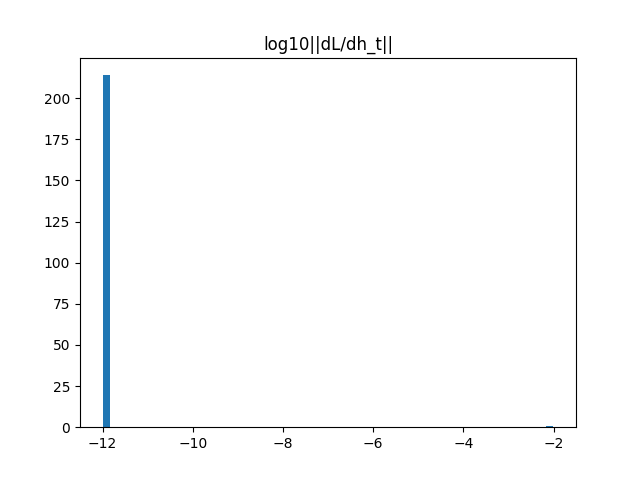
\includegraphics[width=\linewidth]{B1_mul_rnn_tanh_noclip_hist.png}\caption{$\log_{10}\|dL/dh_t\|$}\end{subfigure}
  \begin{subfigure}{0.32\textwidth}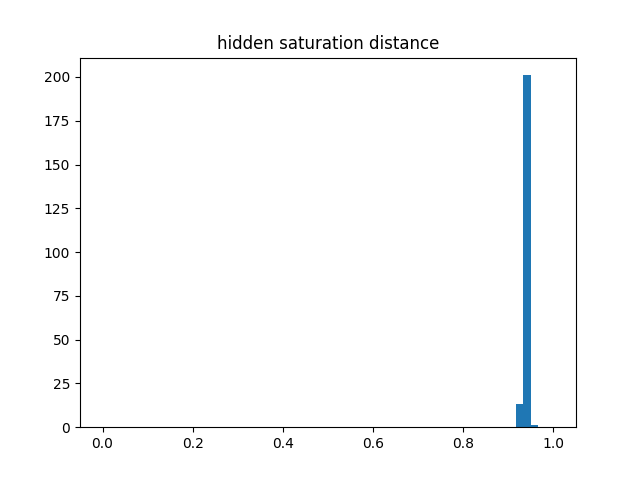
\includegraphics[width=\linewidth]{B1_mul_rnn_tanh_noclip_hidden_sat_dist.png}\caption{hidden sat distance}\end{subfigure}
  \begin{subfigure}{0.32\textwidth}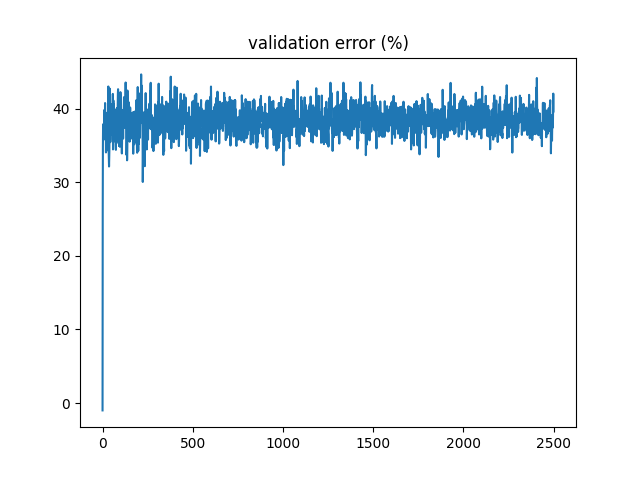
\includegraphics[width=\linewidth]{B1_mul_rnn_tanh_noclip_val_err.png}\caption{valid error}\end{subfigure}
  \caption{B1 diagnostics.}
  \label{fig:b1}
\end{figure}
\noindent\textbf{Q1:} the histogram is essentially a spike at $\log_{10}\|dL/dh_t\|\approx -12$, indicating extreme vanishing gradient-through-time.\\
\textbf{Q2:} hidden saturation distance is near $0.94$ (i.e.\ $|h|\approx 0.06$), so the hidden state is \emph{not} saturated; instead it is very close to $0$ (linear region).
This is a clear counterexample where vanishing gradients occur without tanh saturation.\\
\textbf{Validation:} validation error fluctuates around $\approx 38$--$42\%$ (best $\approx 25.9\%$), indicating limited learning progress in this regime.

\subsection{B2: GRU, no clipping (gate diagnostics)}
\begin{figure}[h]
  \centering
  \begin{subfigure}{0.32\textwidth}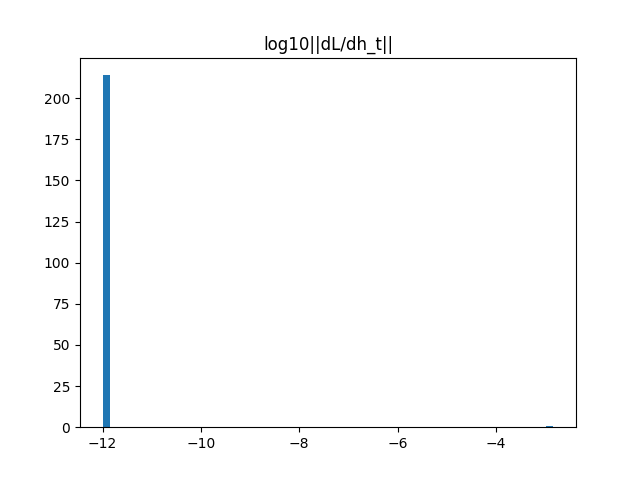
\includegraphics[width=\linewidth]{B2_mul_gru_noclip_hist.png}\caption{$\log_{10}\|dL/dh_t\|$}\end{subfigure}
  \begin{subfigure}{0.32\textwidth}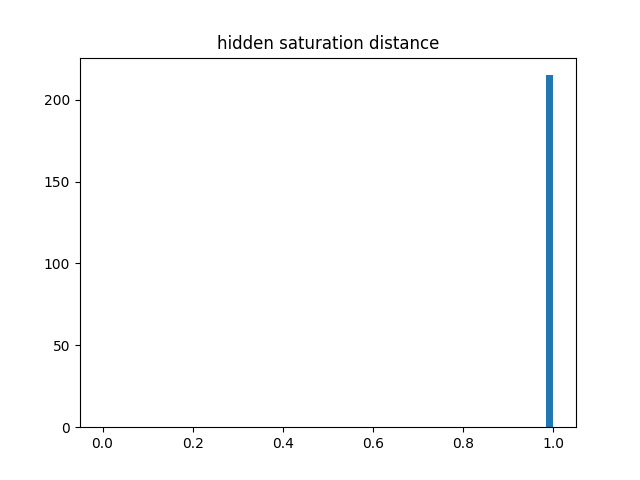
\includegraphics[width=\linewidth]{B2_mul_gru_noclip_hidden_sat_dist.png}\caption{hidden sat distance}\end{subfigure}
  \begin{subfigure}{0.32\textwidth}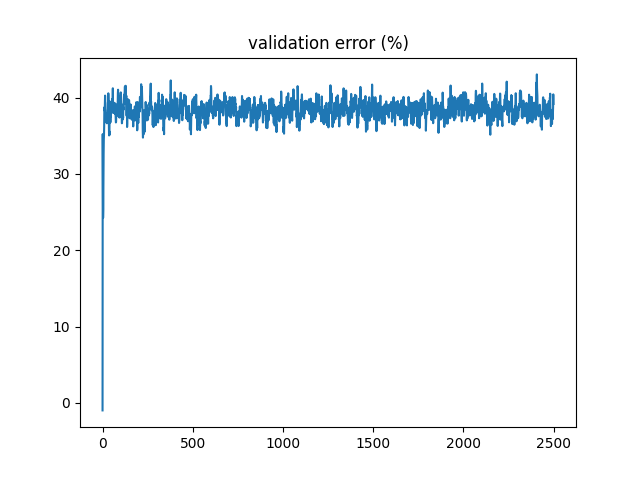
\includegraphics[width=\linewidth]{B2_mul_gru_noclip_val_err.png}\caption{valid error}\end{subfigure}
  \caption{B2 diagnostics.}
  \label{fig:b2}
\end{figure}
\noindent\textbf{Q1:} like B1, the gradient-through-time signal is extremely vanishing (median $\approx -12$).\\
\textbf{Q2:} hidden saturation distance is even closer to $1$ (mean $\approx 0.995$), so hidden activations are very close to $0$.\\
\textbf{Q4 (gate saturation):} Figure~\ref{fig:b2gates} shows $d(z_t)\approx 0.119$ (update gate more saturated) and $d(r_t)\approx 0.499$ (reset gate almost perfectly unsaturated).
Despite gating, the long-range regression signal still collapses over time in this configuration.\\
\textbf{Validation:} validation error is similar to B1 (best $\approx 24.25\%$; final $\approx 39\%$).

\begin{figure}[h]
  \centering
  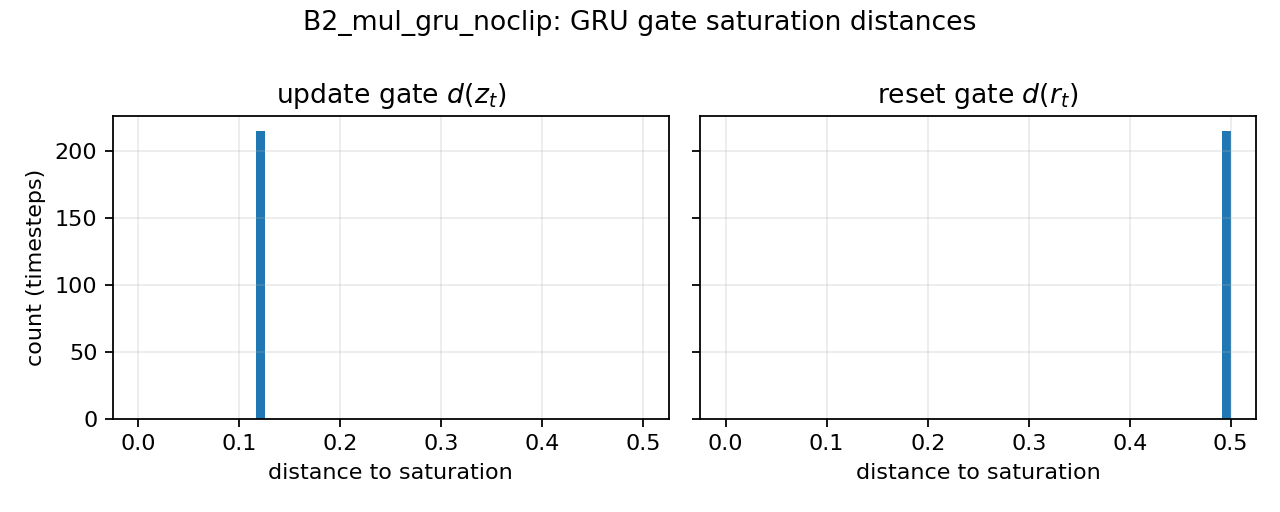
\includegraphics[width=0.85\textwidth]{B2_mul_gru_noclip_gate_sat_hist.png}
  \caption{B2 GRU gate saturation-distance histograms.}
  \label{fig:b2gates}
\end{figure}

\clearpage
\section{Comparisons (Q3--Q5)}

\subsection*{Q3: No clipping vs clipping}
\textbf{RNN on memorization (A1 vs A2/A3):}
\begin{itemize}
  \item \textbf{Gradient norm:} A2 shows very large pre-clip global norms (median $\approx 40.8$), implying parameter-gradient explosion that is subsequently clipped (post-clip norm fixed at the cutoff).
  In contrast, A1 has modest median grad norms but very large $\rho(W_{hh})$ (Figure~\ref{fig:memrho}), indicating unstable recurrent dynamics and saturation.
  \item \textbf{$\log_{10}(g_t)$ histogram:} clipping slightly shifts the distribution (A2/A3 more mass around $\approx -4.6$), but none of A1--A3 reaches the extreme vanishing regime.
  \item \textbf{Saturation:} clipping removes strong tanh saturation (A1: sat-distance near $0$; A2/A3: sat-distance around $0.6$).
\end{itemize}
\textbf{GRU on memorization (A4 vs A5):} clipping moves $g_t$ from clearly vanishing (A4 median $\approx -6.1$) to much healthier values (A5 median $\approx -4.2$), and makes hidden activations strongly unsaturated (A5 sat-distance $\approx 0.85$). Despite these improvements, validation error remains $100\%$ for both.

\begin{figure}[h]
  \centering
  \begin{subfigure}{0.32\textwidth}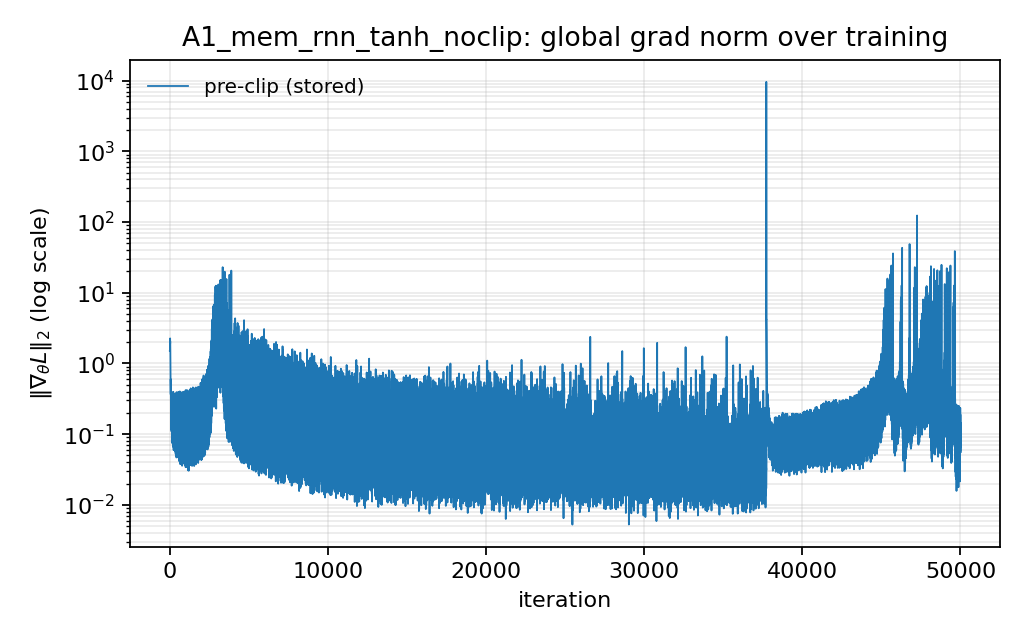
\includegraphics[width=\linewidth]{A1_mem_rnn_tanh_noclip_grad_norm.png}\caption{A1 (no clip)}\end{subfigure}
  \begin{subfigure}{0.32\textwidth}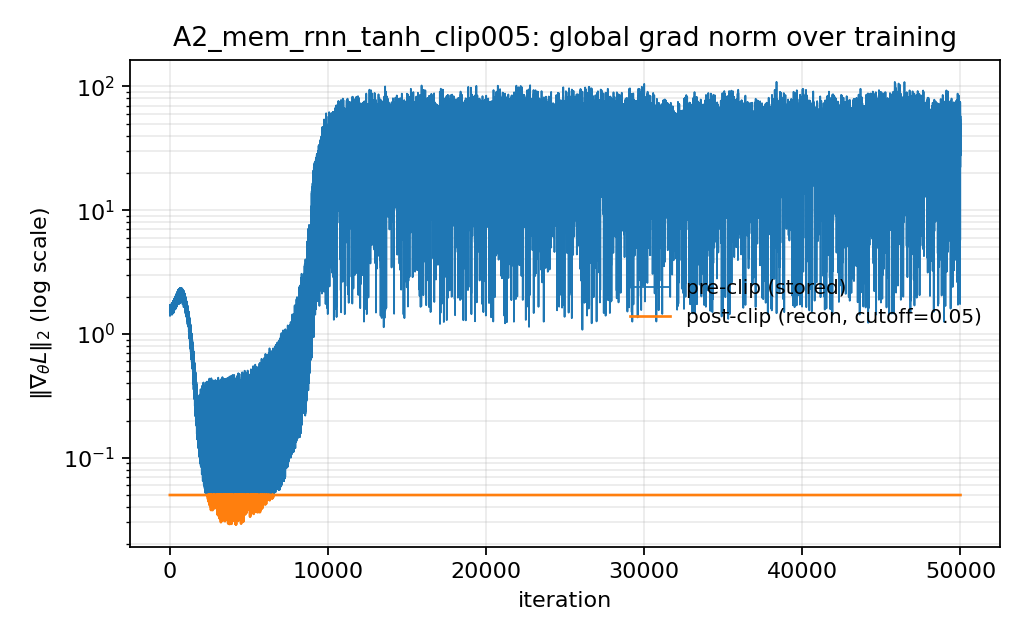
\includegraphics[width=\linewidth]{A2_mem_rnn_tanh_clip005_grad_norm.png}\caption{A2 (cutoff 0.05)}\end{subfigure}
  \begin{subfigure}{0.32\textwidth}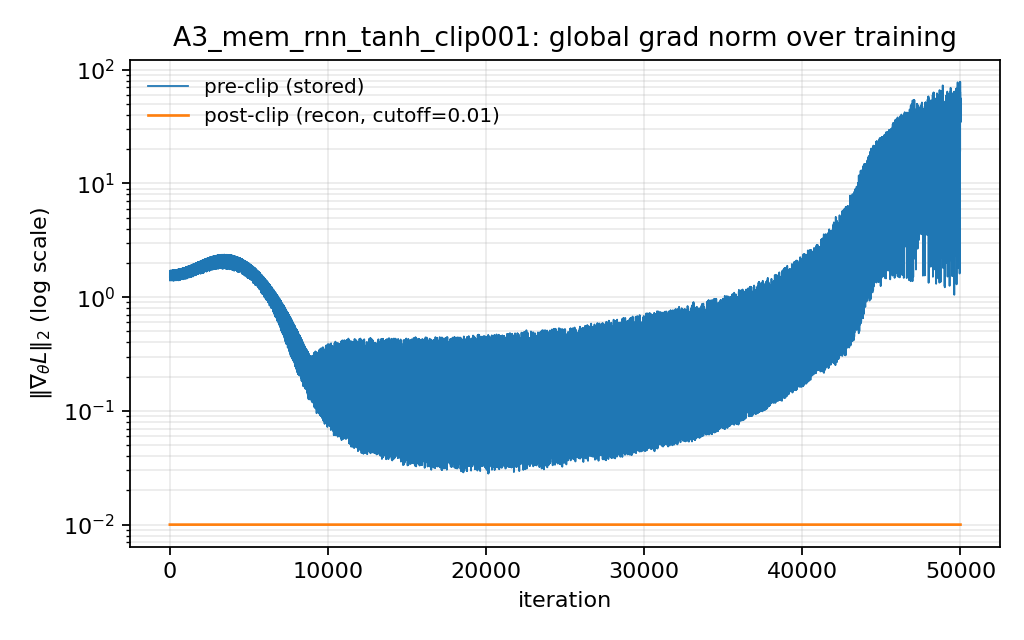
\includegraphics[width=\linewidth]{A3_mem_rnn_tanh_clip001_grad_norm.png}\caption{A3 (cutoff 0.01)}\end{subfigure}
  \caption{Memorization RNN: global gradient norm over training (log scale). For clipped runs, the reconstructed post-clip norm (orange) is capped at the cutoff.}
  \label{fig:rnnmemgradnorm}
\end{figure}

\begin{figure}[h]
  \centering
  \begin{subfigure}{0.49\textwidth}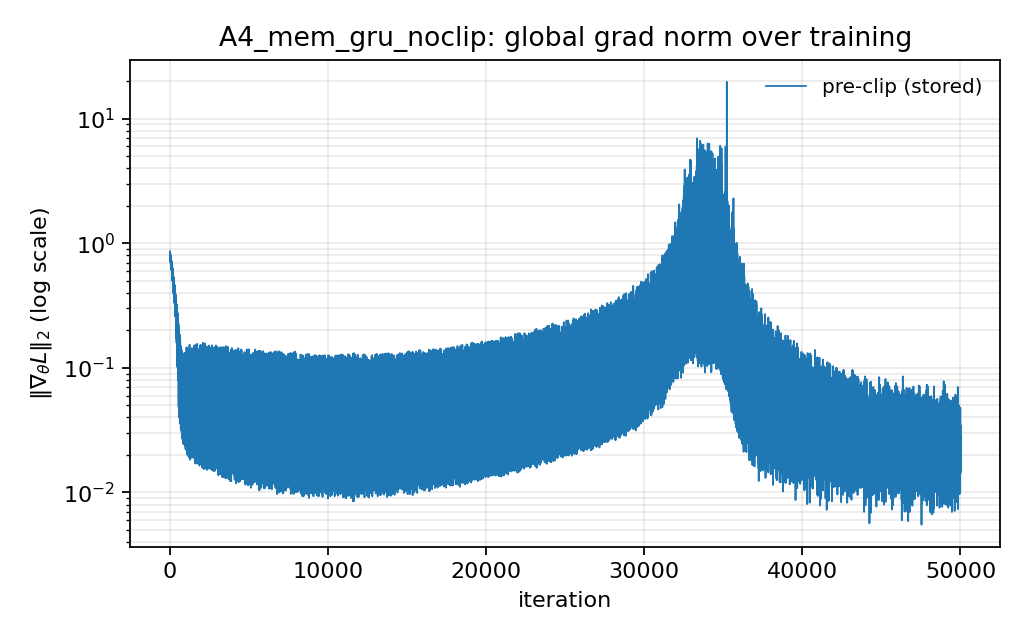
\includegraphics[width=\linewidth]{A4_mem_gru_noclip_grad_norm.png}\caption{A4 (no clip)}\end{subfigure}
  \begin{subfigure}{0.49\textwidth}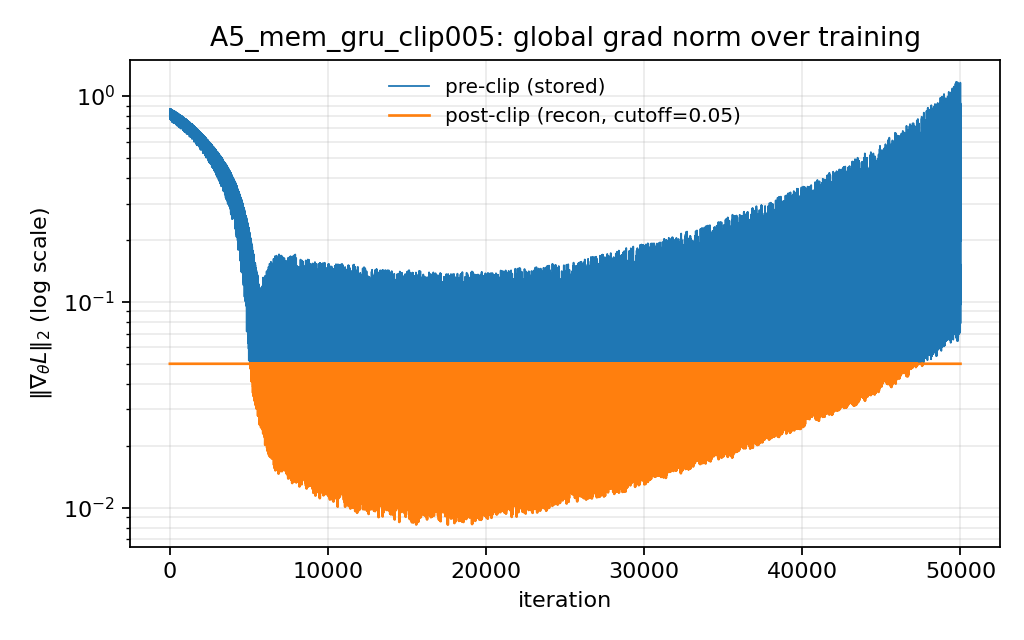
\includegraphics[width=\linewidth]{A5_mem_gru_clip005_grad_norm.png}\caption{A5 (cutoff 0.05)}\end{subfigure}
  \caption{Memorization GRU: global gradient norm over training (log scale).}
  \label{fig:grumemgradnorm}
\end{figure}

\subsection*{Q4: RNN vs GRU (including gates)}
\begin{itemize}
  \item \textbf{Memorization:} the unclipped GRU (A4) exhibits stronger gradient vanishing than the unclipped RNN (A1), even though the RNN has more hidden saturation. Gate diagnostics show the reset gate is largely unsaturated ($d(r_t)\approx 0.46$--$0.49$), while the update gate is more saturated ($d(z_t)\approx 0.12$--$0.18$).
  \item \textbf{Multiplication:} both RNN and GRU collapse to extreme vanishing ($\log_{10}(g_t)\approx -12$) while remaining unsaturated, so the dominant failure mode here is not tanh saturation but the long-range gradient decay inherent to the task and this configuration.
  \item \textbf{GRU-specific failure modes (observed):} the update gate tends to be saturated (low $d(z_t)$), which can reduce effective state updates and make it hard to route precise long-range information; in B2, gating does not prevent vanishing gradients for the long-range regression signal.
\end{itemize}

\subsection*{Q5: $\rho(W_{hh})$ over training and correlation}
Figure~\ref{fig:memrho} and Figure~\ref{fig:mulrho} summarize $\rho(W_{hh})$:
\begin{itemize}
  \item In A1, $\rho(W_{hh})$ grows very large ($\approx 14$) and the network becomes heavily saturated; this correlates with unstable dynamics and failure to learn.
  \item With clipping (A2/A3/A5), $\rho(W_{hh})$ stays close to $1$--$1.3$, consistent with stabilizing updates and reducing saturation/explosion risk.
  \item In B1/B2, $\rho(W_{hh})<1$ (especially B2 where $\rho\approx 0.08$) indicates strongly contractive recurrence; this aligns with the extreme vanishing gradients seen in the $\log_{10}(g_t)$ histograms.
\end{itemize}

\begin{figure}[h]
  \centering
  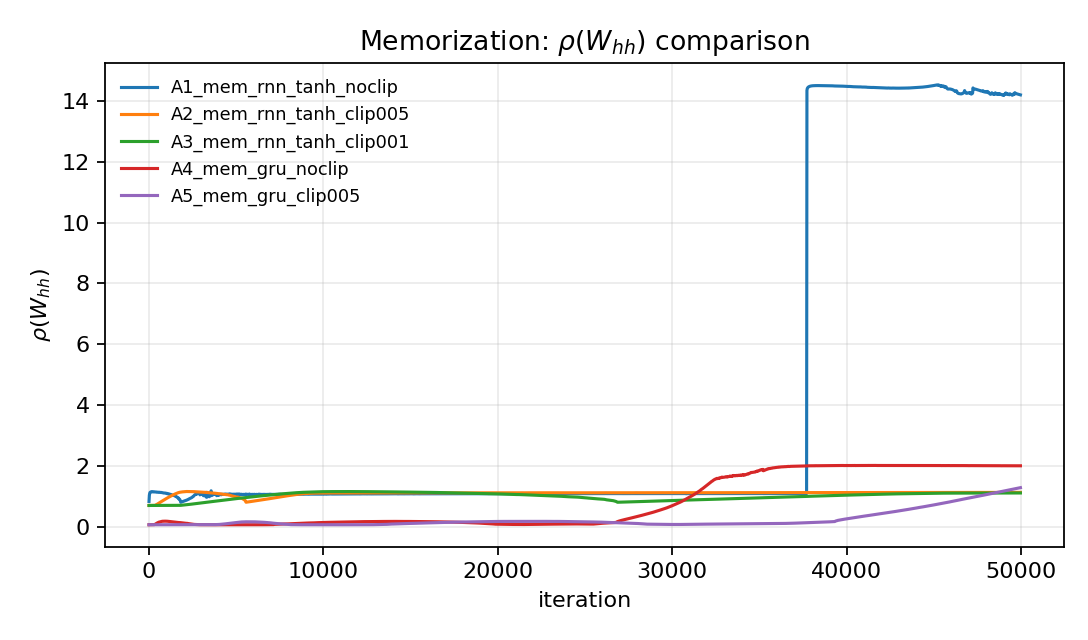
\includegraphics[width=0.95\textwidth]{mem_rho_compare.png}
  \caption{Memorization runs: $\rho(W_{hh})$ over training (all A1--A5).}
  \label{fig:memrho}
\end{figure}

\begin{figure}[h]
  \centering
  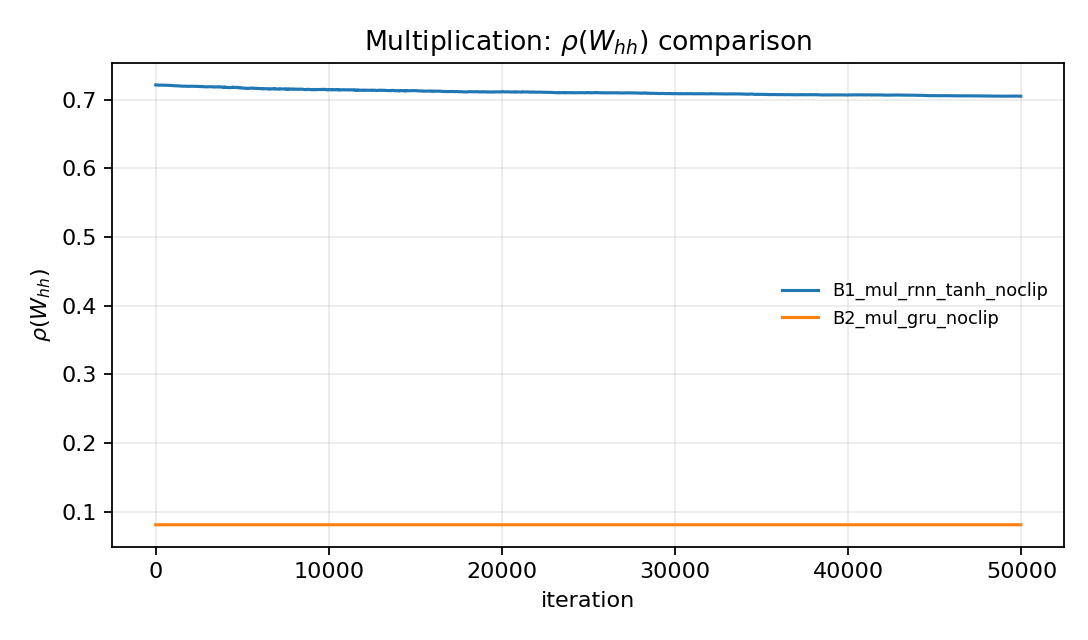
\includegraphics[width=0.95\textwidth]{mul_rho_compare.png}
  \caption{Multiplication runs: $\rho(W_{hh})$ over training (B1--B2).}
  \label{fig:mulrho}
\end{figure}

\clearpage
\appendix
\section{Commands (from assignment PDF)}
The required commands (as provided in the PDF) are reproduced here for completeness:
\begin{verbatim}
# Common flags:
--nhid 50 --lr 0.01 --bs 20 --min_length 50 --max_length 200
--maxiters 50000 --ebs 10000 --cbs 1000 --checkFreq 20
--seed 52 --valid_seed 12345 --collectDiags --diagBins 60 --satThresh 0.05

# A1: mem, RNN tanh, no clipping
python -m trainingRNNs_torch.train --task mem --model rnn --alpha 0.0 \
  --clipstyle nothing --name A1_mem_rnn_tanh_noclip [common flags...]

# A2: mem, RNN tanh, clipping cutoff 0.05
python -m trainingRNNs_torch.train --task mem --model rnn --alpha 0.0 \
  --clipstyle rescale --cutoff 0.05 --name A2_mem_rnn_tanh_clip005 [common flags...]

# A3: mem, RNN tanh, clipping cutoff 0.01
python -m trainingRNNs_torch.train --task mem --model rnn --alpha 0.0 \
  --clipstyle rescale --cutoff 0.01 --name A3_mem_rnn_tanh_clip001 [common flags...]

# A4: mem, GRU, no clipping, with gate diagnostics
python -m trainingRNNs_torch.train --task mem --model gru --alpha 0.0 \
  --clipstyle nothing --diagGates --name A4_mem_gru_noclip [common flags...]

# A5: mem, GRU, clipping cutoff 0.05, with gate diagnostics
python -m trainingRNNs_torch.train --task mem --model gru --alpha 0.0 \
  --clipstyle rescale --cutoff 0.05 --diagGates --name A5_mem_gru_clip005 [common flags...]

# B1: mul, RNN tanh, no clipping
python -m trainingRNNs_torch.train --task mul --model rnn --alpha 0.0 \
  --clipstyle nothing --name B1_mul_rnn_tanh_noclip [common flags...]

# B2: mul, GRU, no clipping, with gate diagnostics
python -m trainingRNNs_torch.train --task mul --model gru --alpha 0.0 \
  --clipstyle nothing --diagGates --name B2_mul_gru_noclip [common flags...]
\end{verbatim}

\section{Reproducibility Notes}
All plots embedded in this report are stored in \texttt{report/images/}.
Additional plots (gradient norm curves, $\rho(W_{hh})$ curves, and GRU gate histograms) were generated from the saved \texttt{*\_final\_state.npz} files using \texttt{report/generate\_extra\_plots.py}.

\end{document}
